\documentclass[a4paper,14pt]{extarticle}
\usepackage{cmap}				% To be able to copy-paste russian text from pdf			
\usepackage[utf8]{inputenc}
\usepackage[T1]{fontenc}
\usepackage[margin=1in]{geometry}
\usepackage[english, russian]{babel}

\usepackage[hyphens]{url}
\urlstyle{same}
\usepackage{hyperref}

\usepackage{multirow}
\usepackage{graphicx}
\usepackage{caption}
\usepackage{amsmath}
\usepackage{mathtools}

\usepackage{tikz}
\usepackage{pgfplots}
\usepgfplotslibrary{groupplots,colorbrewer,dateplot,statistics}

%\def\ishtml{1}
\ifdefined\ishtml
  % HTML mode
  \newcommand{\urlnote}[2]{\href{#2}{#1}} % Make cool link 
  \newcommand{\smallsep}{thinspace} % to be replaced with unicode 8239 later
\else
  % PDF mode
   \usepackage{libertine}
   \usepackage{libertinust1math}
   \newcommand{\urlnote}[2]{#1\endnote{\url{#2}}}  % Put URLs to endnotes
   \newcommand{\smallsep}{\kern 0.1em}
\fi

% Move footnotes to end of document
\usepackage[backref=true]{enotez}
\DeclareTranslation{russian}{enotez-title}{Примечания}

\usepackage[
	output-decimal-marker={,},
	group-separator={\smallsep},
	group-minimum-digits=3
]{siunitx}

% Shoot me if I know a better way to make decimal groups of two
\newcommand{\rateone}[1]{\num{#1}}
\newcommand{\ratetwo}[2]{\num{#1}\smallsep#2}
\newcommand{\ratethree}[3]{\num{#1}\smallsep#2\smallsep#3}

\newcommand{\ru}[1]{\begin{otherlanguage}{russian}#1\end{otherlanguage}}
\newcommand{\en}[1]{\begin{otherlanguage}{english}#1\end{otherlanguage}}
\newcommand{\ruen}[2]{#1 (\en{#2})}

\usepackage[style=alphabetic, backend=biber]{biblatex}
\addbibresource{index.bib}
\renewcommand*{\bibfont}{\small}
\setcounter{biburllcpenalty}{9000}
\setcounter{biburlucpenalty}{9500}

\author{Артём Бакулин}
\date{\today}
\title{Микроструктура рынка и неблагоприятный отбор}

\begin{document}

\maketitle
\thispagestyle{empty}

\begin{figure}[h]
\centering
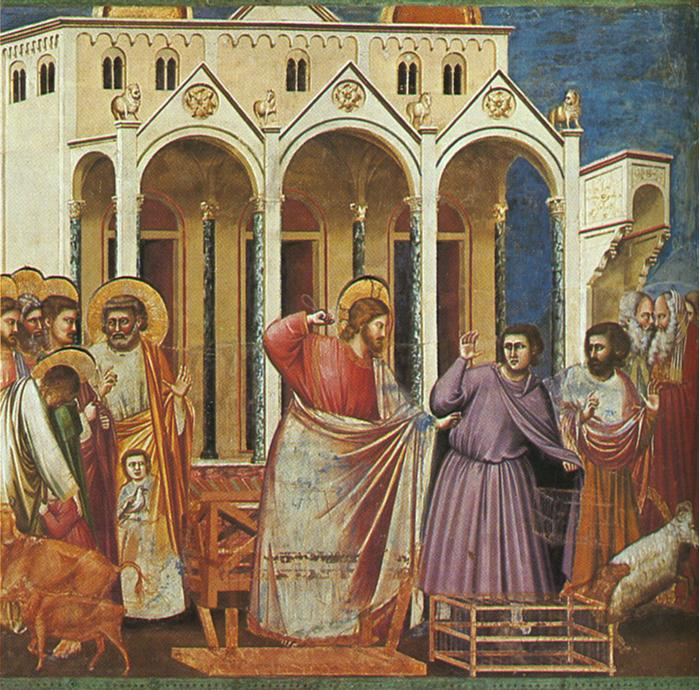
\includegraphics[scale=0.63]{temple.jpg}
\captionsetup{labelformat=empty}
\caption{\small{
Джотто ди Бондоне. \urlnote{Изгнание менял из храма}
{https://commons.wikimedia.org/wiki/File:Giotto_-_Scrovegni_-_-27-_-_Expulsion_of_the_Money-changers_from_the_Temple.jpg}.
ок. 1305 г. Капелла Скровеньи, Падуя.
}}
\end{figure}
\newpage

\section*{Введение}

В предыдущей статье мы выяснили, как работает внебиржевой валютный рынок.
Крупные инвестиционные банки, которые называются дилерами или маркет-мейкерами,
предлагают клиентам курсы покупки и продажи. Клиент покупает валюту дороже
рыночного мид-курса, а продаёт дешевле мид-курса, поэтому на каждой транзакции
он неявно платит дилеру половину спреда. У критично настроенного читателя могли
возникнуть вопросы. Зачем вообще нужны эти маркет-мейкеры? За какую такую услугу
компании реального сектора платят банкам?

Стандартное объяснение из учебников: маркет-мейкер обеспечивает ликвидность
рынка, то есть возможность заключить сделку здесь и сейчас \cite[p.
159,223]{hull2015options}. Представьте, что вы пришли в обменник купить
\num{500} евро, а вас попросили подождать, пока не зайдёт человек, готовый
продать евро. Прямо скажем, не самый лучший сервис. Маркет-мейкер (в данном
случае, обменник) становится стороной сделки и избавляет вас от необходимости
ждать или, чего доброго, садиться на телефон и обзванивать знакомых в поисках
потенциального продавца.

На это можно возразить, что человечество давно придумало биржи, электронные
книги заявок и центральных контрагентов. Если все компании будут отправлять свои
заявки на покупку и продажу на биржу, то найти контрагента по сделке будет
нетрудно.

У меня есть несколько соображений на этот счёт. Во-первых, даже на биржах нужны
маркет-мейкеры, которые держат в книге заявок свои заявки на покупку и на
продажу, увеличивая ликвидность рынка. Их роль настолько важна, что биржи часто
выплачивают маркет-мейкерам вознаграждение сверх тех денег, которые они
зарабатывают на спреде \cite{moex2018mm}\cite[ch. 7]{hasbrouck2017securities}.
Если маркет-мейкер всё равно необходим, то не лучше ли, чтобы клиенты обращались
к нему напрямую? Зачем вводить дополнительного посредника в лице биржи, которая
тоже хочет заработать комиссию?

Во-вторых, в прошлый раз вы могли убедиться, что оптимальное исполнение сделок в
книге заявок --- не самое простое дело. Чем больше размер желаемой сделки, тем
больше спреда вы заплатите, потому что вы будете <<съедать>> всё больше уровней
книги заявок по всё более невыгодному курсу. Если же присоединиться к очереди со
своей заявкой чуть выгоднее мид-курса, то есть риск упустить момент и опоздать
со сделкой. Найти правильный баланс между заплаченным спредом и
неопределённостью времени исполнения не так-то легко. Банк, помимо прочего,
продаёт клиентам свою экспертизу в этом вопросе. Банк может предложить клиенту
цену выгоднее, чем та, что он заплатит, если прямолинейно исполнит сделку в
книге заявок. После сделки вопрос оптимальной стратегии торговли становится
головной болью трейдеров и программистов из банка, а не клиента.

Что мог бы ответить критик? Если на биржевом рынке не хватает ликвидности, то не
потому ли, что банки используют своё уникальное положение и не дают ему
развиваться? В конце концов, сами-то банки торгуют на межбанковском рынке именно
через книгу заявок. Возможно, если преодолеть лобби банков-дилеров и сделать
биржи более доступными, то заявок продавцов и покупателей из реального сектора
хватит, чтобы получился ликвидный рынок с узкими спредами.

Чтобы ответить и на этот вопрос, нам придётся углубиться в область экономики,
которая называется \ruen{микроструктура рынка}{market microstructure}.

\section*{Рынок кредитных деривативов}

Давайте посмотрим на естественный эксперимент, который разворачивается на наших
глазах в течение последних шести лет. После кризиса 2008-го года в США был
принят \ruen{закон Додда--Франка}{Dodd--Frank Act}, который, среди прочего,
реформировал рынок (только не пугайтесь длинного названия!) \ruen{индексных
кредитных дефолтных свопов}{index credit default swap} \cite{collin2018}.

Экономическая суть этих свопов совершенно не важна для нашего сегодняшнего
обсуждения, поэтому не страшно, если вы не знаете, что это такое. Важно, что
реформа почти полностью прекратила внебиржевую торговлю этими инструментами в
США. За редким исключением, купить или продать индексный кредитный дефолтный
своп можно только на специальных электронных площадках, которые называются
\en{Swap Execution Facility (SEF)}. Самые известные из них ---
\urlnote{Bloomberg}{https://www.bloomberg.com/professional/product/swap-execution-facility/}
и
\urlnote{TradeWeb}{https://www.tradeweb.com/our-markets/market-regulation/sef/}.

Каждый SEF поддерживает несколько способов заключения сделок. Первый способ
называется request for stream (RFS). Клиент вводит детали свопа и просит кого-то
из подключенных к системе дилеров регулярно присылать ему в терминал свежие
<<индикативные>> цены. Индикативность цены означает, что когда клиент щёлкнет по
ней мышкой, чтобы заключить сделку, дилер может как согласиться, так и отклонить
запрос. Похоже на рынок аренды, когда вы звоните по объявлению, а вам говорят,
что квартира уже сдана, но в соседнем подъезде есть похожая.

Второй способ называется \en{request for quote (RFQ)}. Клиент отмечает галочками
несколько (по закону --- не меньше трёх) дилеров и устраивает аукцион. Дилеры
присылают свои котировки на интересующий клиента своп, чтобы он выбрал лучшее
предложение. Обычно цены на аукционе являются \ruen{<<твёрдыми>>}{firm}, и дилер
не имеет права отказаться от сделки, если клиент выберет именно его. И в случае
RFS, и в случае RFQ клиент может попросить как одностороннюю котировку (только
на покупку или только на продажу), так и двухстороннюю.

Третий способ --- книга лимитных заявок. Закон обязывает каждый SEF вести книгу
заявок, чтобы любая компания могла отправить лимитную заявку на покупку или
продажу свопа. Законодатели также постановили, что в сделках с наиболее
ликвидными индексными свопами всегда участвует центральный контрагент. Благодаря
этому все могут торговать со всеми и не опасаться кредитного риска.

Все три способа заключения сделок имеют аналоги на валютном рынке. Механизмы RFS
и RFQ похожи на общение клиента и маркет-мейкера на внебиржевом рынке. RFS это
взаимодействие напрямую, а RFQ --- через многодилерскую платформу. Книга заявок
и сделки с центральным контрагентом один в один повторяют биржевой рынок.

Что бы вы думали? И по сей день в подавляющем большинстве случаев участники
рынка предпочитают заключать сделки с помощью RFS и RFQ, а не через книгу
заявок. Возможно ли, что профессионалы, которые по меньшей мере знают, что такое
индексный кредитный дефолтный своп, не понимают своего счастья и обращаются к
дилерам исключительно в силу инерции мышления? Давайте не будем рассматривать
эту гипотезу всерьёз. Лучше повнимательнее почитать правила торгов, и тогда
выяснится, что у клиентов могут быть вполне рациональные мотивы обращаться к
дилерам, а не пользоваться книгой заявок.

\section*{Анонимность и информированность}

Принципиальное отличие книги заявок от RFS и RFQ --- анонимность. Только
торговая площадка, то есть SEF, знает, кто отправил ту или иную заявку, а для
всех участников рынка это тайна. Они видят, что кто-то готов купить своп по 42,
но они не знают, кто это --- крупный инвестбанк или <<Рога унд копыта АГ>>. В
механизме RFS и RFQ анонимность не предусмотрена. Все дилеры видят название
клиента, который отправил им запрос. Казалось бы, сущая мелочь, но эта мелочь
имеет неожиданные последствия. Раскрыв своё имя, многие клиенты могут получить
более выгодное предложение от дилеров.

Предположим, что всех клиентов можно разделить на две категории: информированных
и неинформированных. Информированные клиенты лучше других умеют предсказывать
краткосрочные движения цен и любят покупать перед ростом цен и продавать перед
падением. Неинформированные клиенты, как можно догадаться, с примерно равной
вероятностью покупают как перед ростом, так и перед падением.

Информированным клиентом может быть алгоритмический хэдж-фонд, который обучил
нейронную сеть читать ленту новостей и торговать в соответствии с полученной
информацией быстрее, чем белковые участники рынка. Пример неинформированного
клиента --- небольшой банк, который раз в месяц покупает чуточку кредитных
дефолтных свопов, чтобы компенсировать риск своего кредитного портфеля.

Поставьте себя на место дилера. С запросом на покупку одного и того же свопа к
вам обратились два клиента: хэдж-фонд и небольшой банк. За последний месяц вы 10
раз торговали с хэдж-фондом, и 8 раз из 10 рынок шёл против вас в течение
нескольких минут после сделки, оставляя вас в убытке. С банком вы торгуете не
так часто, раз в пару месяцев, и за последний год вы ни разу не теряли деньги на
его сделках. Внимание, вопрос. При прочих равных, кому из этих клиентов вы
предложите цену ниже, а кому выше?
 
Мне кажется, что в такой постановке задачи ответ очевиден. Имеет смысл дать
лучшую цену небольшому банку, потому что это позволит выиграть аукцион. Можно
ожидать, что через несколько минут другой клиент придёт к вам, чтобы продать
своп, и тогда вы почти без риска заработаете на спреде между покупкой и
продажей. Напомню, что небольшой банк --- не из тех, кто систематически покупает
перед ростом рынка. Каждая отдельная сделка может обернуться против вас, но если
у вас достаточно неинформированных клиентов, то на дистанции вы будете
зарабатывать деньги.

Как насчёт запроса от хэдж-фонда? Будет разумным назначить ему цену чуть выше.
Основываясь на предыдущем опыте, сразу после сделки вам придётся бежать на
рынок, чтобы успеть купить своп до вероятного роста цен. Придётся заплатить
спред другому дилеру, так что пусть хэдж-фонд компенсирует вам эти расходы. Если
же вы по какой-то причине не сможете или не захотите идти на рынок, а цена свопа
всё-таки начнёт расти, то пусть у вас будет какой-никакой запас прочности, и вы
начнёте нести потери при большем движении цен. Глядишь, и обойдётся --- рынок
сдвинется вверх, но вы продадите клиенту своп настолько дорого, что рынок не
дойдёт до этой цены, и вы всё равно останетесь в плюсе.

Объяснение на пальцах кажется разумным, на то оно и <<на пальцах>>. Как
проверить гипотезу, что дилеры предлагают клиентам разные цены в зависимости от
степени их информированности? Исследователи проанализировали множество реальных
сделок и вычислили для каждой из них два параметра. Первый параметр --- спред,
который заплатил клиент, когда купил своп дороже мид-курса или продал своп
дешевле мид-курса. Второй --- изменение рыночного мид-курса в течение 15 минут
после заключения сделки.

В среднем, если случайно выбранный клиент покупает своп у дилера, то в течение
15 минут после сделки рыночная цена свопа обычно растёт, а если клиент продаёт
своп дилеру, то рыночная цена после сделки снижается. В обоих случаях изменение
цены работает в пользу клиента и против дилера. Это подтверждает, что среди
клиентов есть информированные. Есть и другая закономерность. При прочих равных,
чем более неблагоприятным для дилера было изменение цены за 15 минут
\emph{после} сделки, тем более широкий спред он прислал в котировке \emph{до}
сделки. Либо дилеры предсказывают будущее, либо они заранее оценивают степень
информированности клиентов и осознанно присылают котировки с широким спредом
наиболее информированным из них.

Таким образом, если клиент не является информированным, то у него есть стимул
отказаться от анонимной книги заявок и предпочесть неанонимный механизм RFS или
RFQ. Замечу, что неинформированность это не обязательно плохо. Если клиент
покупает или продаёт свопы не для того, чтобы заработать на краткосрочном
колебании цены, а для управления рисками своего основного бизнеса, то он не
воспринимает собственную неинформированность как недостаток. Это скорее
преимущество, которое позволяет получить от дилеров котировки с более узким
спредом и тем самым снизить расходы на сделки.

\section*{Неблагоприятный отбор}

Продолжим изучать рынок индексных кредитных дефолтных свопов. Интересно, что
разделение рынка на два сегмента, междилерский и клиентский, сохранилось и после
реформы. Клиенты торгуют с дилерами на одних SEF'ах, таких как упомянутые выше
\en{Bloomberg}\ и \en{TradeWeb}, а дилеры торгуют между собой на других,
например на \urlnote{GFI Swaps
Exchange}{http://www.gfigroup.com/markets/gfi-sef/overview/}. Как мы уже знаем,
клиенты предпочитают механизмы RFS и RFQ. Дилеры же чаще пользуются книгой
заявок или другими похожими анонимными механизмами.

Во введении к статье я упомянул, что дилер может предложить клиенту цену лучше,
чем в междилерской книге заявок. Кому-то это утверждение могло показаться
необоснованным. Ситуация на рынке свопов подтверждает, что это возможно. В 95\%
(!) случаев клиенты получают от дилеров котировки выгоднее, чем в книге заявок
\en{GFI Swaps Exchange}, то есть дороже лучшей заявки на покупку и дешевле
лучшей заявки на продажу.

В этом нет ничего удивительного. Если из-за анонимности книги заявок невозможно
предвидеть, с кем будет заключена сделка, то все участники неизбежно вкладывают
в цены риск заключить невыгодную сделку с кем-то более информированным. 

Рассмотрим пример. У вас есть возможность выставить заявку на покупку некоторого
актива (скажем, того же свопа). Вы знаете, что в будущем актив может стоить
либо 95 рублей, либо 105 рублей с вероятностью 50/50. После того, как вы
выставите заявку, на рынок придёт неинформированный продавец, который продаст
вам актив по указанной вами цене. После сделки мы также выясним, какой из двух
случайных исходов реализовался, то есть стоит ли актив 95 или 105. Если вы купите
актив дешевле финальной цены, то вы выиграли. Например, если окажется, что актив
стоит 105 рублей, а вы выставили заявку с ценой 98, то вы заработаете 7 рублей.

Какую цену вы должны указать в заявке на покупку, чтобы в среднем по крайней
мере не терять деньги? Не нужно заканчивать мехмат, чтобы сообразить, что
математическое ожидание прибыли равно нулю при цене покупки $(95+105)/2 = 100$ .
Если вы будете раз за разом играть в эту игру и заявлять цену 100, то вы не будете ни
терять, ни зарабатывать. Если вы не единственный покупатель на рынке, то конкуренция
заставит вас выставить цену достаточно близко к равновесной --- либо ровно 100, либо
на копеечку ниже.

Теперь изменим правила игры. Предположим, что продавец будет неинформированным
с вероятностью не 100\%, а только 90\%. С вероятностью 10\% на рынок придёт 
информированный продавец, который совершенно точно знает, стоит ли актив 95 или
105. Информированный продавец заключит с вами сделку только если она ему выгодна.
Например, если вы выставите заявку с ценой 100, то он продаст вам актив, только если 
его будущая цена равна 95. Если вы выставили заявку с ценой 100, а актив на самом деле
стоит 105, то информированный продавец просто откажется от сделки, и ваша прибыль
будет равна нулю.

Если аккуратно расписать вероятности на бумажке, то нетрудно вычислить, что новая 
равновесная цена заявки, при которой вы не будете ни терять, ни зарабатывать, равна 
$$\frac{0.5\cdot95 + 0.5\cdot(1-0.1)\cdot105}{0.5 + 0,5\cdot(1-0.1)} \approx 99.74$$

Другими словами, присутствие информированного продавца приводит к тому,
что вы должны указать в заявке цену на 26 копеек ниже той равновесной цены,
которая установилась бы на рынке, если бы все участники обладали одинаковой
информацией. Эта поправка к цене лимитных заявок называется \ruen{стоимостью неблагоприятного
отбора}{adverse selection cost}. Её точное значение зависит от многих
параметров, в том числе от доли информированных участников рынка и степени их
осведомлённости. Если вам интересно, то формальные модели можно посмотреть в
\cite[ch. 11]{hasbrouck2017securities} или \cite[ch. 6]{foucault2013market}.

Если волевым решением запретить дилерский рынок и согнать всех в книгу заявок,
то будут и выигравшие, и проигравшие. Сейчас каждый платит дилерам
индивидуальную цену неблагоприятного отбора в соответствии с собственной
информированностью, а в объединённой книге заявок эта цена будет равномерно
распределена на всех. Средний спред в книге заявок будет хуже, чем тот, который
неинформированные клиенты привыкли получать от дилеров, но лучше, чем защитный
спред, который дилеры предлагали информированным спекулянтам. Действительно ли
это то, что мы хотим --- снизить транзакционные издержки спекулянтов за счёт
компаний, которые используют деривативы по прямому назначению, для управления
рисками?

\section*{Проклятие победителя}

Раз уж мы начали говорить об аукционах RFQ, не могу не упомянуть ещё один
интересный факт. Несмотря на то, что к SEF-ам подключены десятки дилеров,
клиенты чаще предпочитают отправить RFQ только трём--пяти из них. Кроме того,
чем крупнее сделка, которую хочет заключить клиент, тем меньше дилеров он
включает в аукцион \cite{riggs2019}. Это противоречит интуиции, которая
подсказывает, что чем выше конкуренция среди дилеров, тем лучше клиенту.

Здесь вступает в игру ещё одна особенность организации торгов. SEF сообщает
дилерам, сколько конкурентов участвует в каждом конкретном аукционе. Почему это
важно, спросите вы? Дело в том, что аукционы с большим количеством участников
подвержены проклятию победителя (winner's curse).

Предположим, что клиент желает купить \num{100500} единиц свопа и добавил в
аукцион сразу 20 дилеров. Чтобы выиграть аукцион, дилер должен предложить цену
ниже, чем 19 его коллег. Однако, если все 20 конкурентов одинаково хорошо
разбираются в рынке, то <<справедливая>> цена свопа скорее будет близка к
\emph{среднему} из их предложений, чем к \emph{минимальному} из них. Победитель
аукциона заберёт себе сделку, но скорее всего предложит клиенту цену ниже, чем
стоило бы.

Получается, что дилеру не выгодно выигрывать аукцион с большим количеством
участников. Из данных о ходе торгов следует, что чем больше участников в
аукционе, тем выше вероятность, что дилер просто не пришлёт свою котировку, и
тем шире спред, который он выставит клиенту, если всё-таки решит участвовать.
Зная это, клиент сам ограничивает количество дилеров тремя--пятью, и это
ограничение конкуренции улучшает цену, которую он в конце концов получает!
Бывает и такое, что некоторые SEF'ы, заботясь о клиентах, на уровне торговой
программы позволяют одновременно выбрать не более пяти--шести дилеров.

\section*{Валютный рынок}

Вернёмся к валютному рынку. Действуют ли на нём те же механизмы, что и на рынке
кредитных свопов? Оценивают ли банки информированность клиентов, которые
обращаются к ним за котировками?

Кевин Роджерс, бывший трейдер в \en{Deutsche Bank}, вспоминает, что он и его
коллеги систематически анализировали сделки клиентов по крайней мере в 2006-м
году \cite[p.~84]{rodgers2016why}. Тогда они обнаружили, что некоторые
хэдж-фонды получали сообщения от EBS на несколько миллисекунд раньше, чем банк,
и пользовались этим. Например, если банк предлагал на своей платформе
\en{AutobahnFX}\ котировку евро-доллар \num{56}--\num{58}, а рынок EBS скачком
двигался к уровню \num{59}--\num{61}, то фонд покупал у банка евро по \num{58} и
тут же продавал их на EBS по \num{59}. Так фонд практически из воздуха
зарабатывал 1 пип, то есть по 100 долларов с каждого миллиона евро.

Такие фонды называют \ruen{снайперами}{snipers}, потому что они постоянно
высматривают и \ruen{отстреливают}{pick off}\ тех маркет-мейкеров, кто
замешкался и не успел обновить котировки. В терминах предыдущего раздела, они,
безусловно, являются информированными клиентами. Судя по открытым источникам,
остальные крупные дилеры тоже много лет инвестируют в системы, анализирующие
сделки клиентов. В результате информированные клиенты получают более широкий
спред, чем безобидные неинформированные \cite{wood2018}.

Помимо спреда, дилеры используют уникальный механизм валютного рынка --- право
на последний взгляд (last look). Когда клиенту нравится цена, предложенная
дилером, и он отправляет запрос на сделку, дилер может подумать несколько
миллисекунд и отказаться. Дилеры вводят такие задержки, чтобы защититься от
<<снайперов>>, эксплуатирующих технологическое преимущество. Это позволяет
показывать всем клиентам более узкий спред, но причиняет страдания наиболее
быстрым участникам рынка, которые иногда упускают возможность заключить выгодную
сделку \cite{cartea2019}.

В статьях \cite{oomen2017} и \cite{oomen2019} Роел Оомен из Deutsche Bank
приводит интересный пример того, как анализ данных помог клиенту и дилеру
договориться о взаимовыгодном сотрудничестве на валютном рынке.

Некий клиент запрограммировал агрегатор ликвидности. Он подключился сразу к
нескольким дилерам и написал код, который в поисках лучшей цены опрашивает всех
подряд и при необходимости дробит сделку между дилерами. По задумке, это должно
было снизить расходы на сделки. На практике вышло по-другому. Со временем клиент
обнаружил, что дилеры предлагают ему слишком широкий спред и часто отклоняют его
сделки, пользуясь правом последнего взгляда. Причина этих бед --- разный подход
дилеров к управлению риском.

В общем случае, заключив сделку с клиентом, дилер может выбрать одну из двух
стратегий поведения. Первая опция --- \ruen{<<переварить>>}{internalise}\ риск.
Например, если дилер продал клиенту доллары за рубли по курсу \num{66.50}, он подождёт
несколько минут, чтобы купить доллары у другого клиента по \num{66.48}. В спокойные
времена, когда рыночная цена не сильно меняется, дилер может заработать полный
спред между курсами покупки и продажи. С другой стороны, дилер рискует потерять
деньги, если рынок сдвинется вверх до того, как к нему обратится второй клиент.

Второй вариант --- <<выплюнуть>> риск на рынок (externalise). Продав доллары за
рубли по курсу \num{66.50}, дилер побежит на рынок (на биржу или к другому
дилеру), чтобы попытаться купить их по \ratetwo{66.49}{95}. Да, он не заработает
полный спред, зато почти сразу избавится от риска. Проблема заключается в том,
что самим своим появлением на рынке дилер может сдвинуть цену. Он же хочет
\emph{купить}, а что бывает, когда покупателей становится больше? Правильно,
цена растёт.

Предположим, что клиент с помощью своего волшебного агрегатора разделил крупную
сделку, скажем, покупку 10 миллионов долларов за рубли, поровну между пятью
дилерами. Четверо из дилеров предпочитают переваривать риск, а пятый ---
выплёвывать его на рынок. Как только пятый дилер вышел на рынок, чтобы купить 2
миллиона долларов за рубли, повышение спроса подтолкнуло рыночную цену вверх.

Клиент может об этом и не догадываться, но как видят ситуацию первые четыре
дилера? Сразу же после того, как клиент купил у них 2 миллиона, рыночная цена
выросла, как будто клиент предвосхитил движение рынка. Если это будет
повторяться достаточно часто, то дилеры пометят клиента как опасного и начнут
выставлять более широкий защитный спред. Вероятно, именно это и произошло в
реальности.

Когда клиент обратился к одному из дилеров, чтобы обсудить ситуацию, ему
предложили контролируемый эксперимент. В течение нескольких недель он
пользовался услугами только этого дилера, чтобы торговать одной из ликвидных
валютных пар. Взамен дилер пообещал показывать узкий спред, никогда не
пользоваться правом последнего взгляда, а также переваривать сделки, а не
выплёвывать их. Случилось чудо: в сделках клиента не оказалось ничего опасного,
и дилер смог стабильно зарабатывать даже на достаточно узком спреде. Клиент
получил возможность не только платить меньше спреда, но и сократить операционные
расходы, потому что обрабатывать сделки с одним дилером проще, чем с пятью.

Как видите, и на валютном рынке дилеры классифицируют клиентов как
информированных или неинформированных. Можно сделать вывод, что сложившаяся
структура внебиржевого валютного рынка выгодна не только банкам-дилерам, но и
значительному числу клиентов. В отсутствие анонимности неинформированные клиенты
могут заключать сделки на более выгодных условиях, чем в анонимной книге заявок.

\section*{Ценовая дискриминация}

Звучит вполне логично, не правда ли? Если мои аргументы показались вам
достаточно убедительными, то поздравляю: вы только что прочитали мнение адвоката
дьявола. К моменту написания этих строк я уже десять лет работаю в банке
и разрабатываю системы, сюрприз-сюрприз, торгующие валютой с клиентами. Моё
личное благосостояние напрямую зависит от того, сможем ли мы в будущем
зарабатывать деньги маркет-мейкерством на внебиржевом рынке валютных
деривативов. Было бы странно, если бы я сейчас вышел весь в белом и заявил, что
всё, чему я отдал лучшие годы своей жизни --- это обман трудящихся и высасывание
соков из реальной экономики. Тем не менее, объективность требует изложить и
другую точку зрения.

В сущности, то, что делают дилеры, в микроэкономике называется ценовой
дискриминацией (price discrimination). Слово <<дискриминация>> здесь не имеет
негативной коннотации и всего-навсего описывает ситуацию, когда продавец
предлагает разным покупателям разные цены на один и тот же товар. Как мы уже
видели, это не обязательно плохо. Часто клиент сам желает быть
дискриминированным, чтобы получить цену лучше, чем в среднем по рынку.

Однако дискриминация может работать и в обратном направлении. Реальность
внебиржевого рынка такова, что только для того, чтобы получить возможность
заключать сделки с новым дилером, нужно ощутимо вложиться --- от бюрократии при
открытии счёта до внесения гарантийного обеспечения. Для многих небольших
компаний это чересчур высокие накладные расходы, поэтому они оказываются
привязаны к одному-единственному банку.

Если клиент не может уйти, то какие у банка стимулы давать ему лучшую цену, то
есть более узкий спред? Да, небольшая компания из реального сектора вряд ли так
же информирована, как хэдж-фонд, и её сделки совершенно безобидны. Теоретически,
банк мог бы показать ей довольно узкий спред, но заработает ли он на этом?

С точки зрения банка, более узкий спред имеет смысл, только если сделок станет
больше. Грубо говоря, лучше заработать трижды по 100 евро на трёх сделках, чем
200 евро на одной. Эта логика прекрасно работает для крупных компаний калибра
Volkswagen или Airbus, которые могут себе позволить поддерживать отношения с
десятком дилеров. Банку выгодно сузить спред в полтора раза (согласиться
зарабатывать в полтора раза меньше на каждой отдельной сделке), если это
позволит заполучить не 10\%, а 20\% валютных сделок этой компании (нарастить
объём сделок в два раза).

Если небольшая компания уже и так продаёт 100\% валютной выручки одному банку,
то можно уменьшить спред хоть до нуля, но объём сделок всё равно не вырастет. У
компании физически нет больше иностранной валюты, чем она зарабатывает. Если
банк улучшит спред для такого клиента, то он упустит прибыль, не получив ничего
взамен.

Происходит ли отрицательная дискриминация на практике? Здесь мы вступаем на
зыбкую почву, потому что банки не обязаны публиковать свои сделки, и у
независимых исследователей не так много данных для анализа. Есть буквально пара
статей, которые описывают отрицательную дискриминацию как на спотовом валютном
рынке \cite{bjonnes2017}, так и на рынке деривативов \cite{hau2019}. Получается,
что небольшие и средние компании платят за обмен валюты едва ли не на порядок
больше (в процентах от размера сделки), чем крупные корпорации и инвестиционные
фонды. При этом степень дискриминации уменьшается, если небольшой клиент
запрашивает котировки у нескольких банков через платформы-агрегаторы.

Чувствую, что уже пора включить режим адвоката дьявола ещё раз. Во-первых, у
меня есть чисто технические замечания к методологии во второй статье, которая
случайно попала в область моей специализации. Насколько я могу судить, авторы не
учитывают стоимость \ruen{кредитного риска}{credit valuation adjustment, CVA}\ и
стоимость капитала, который банк обязан зарезервировать под сделку (\en{capital
valuation adjustment, KVA}\endnote{Буква K как в <<Das Kapital>>. Буква C уже
занята в сокращении credit valuation adjustment (CVA).}). Эти поправки к цене
сделки с небольшой компанией без кредитного рейтинга действительно могут быть на
порядок больше, чем спред, который заплатил бы надёжный клиент с высоким
кредитным рейтингом. Это не упрёк авторам работы: имеющиеся у них данные в
принципе не позволяют вычислить эти компоненты спреда.

Во-вторых, есть и более общий аргумент. Когда по дороге на работу я покупаю
мороженое в <<Азбуке вкуса>>, мне и в голову не приходит возмутиться, что
розничная цена за один стаканчик выше, чем цена точно такого же стаканчика в
оптовой партии из 100 ящиков. Такова жизнь: оптом --- дешевле. Банки вкладывают
в спред не только стоимость рыночного риска, но и операционные издержки на
обработку сделок. Некоторые издержки, такие как рабочее время персонала, не
зависят от размера сделки. Поэтому нет ничего удивительного в том, что банки
дают скидки крупным клиентам, позволяя им реализовать экономию от масштаба. Я
думаю, что по мере того, как автоматизация будет сокращать расходы на проведение
транзакций, небольшие клиенты тоже увидят более узкие спреды.

\section*{Заключение}

Как показывает естественный эксперимент на рынке кредитных свопов, даже если у
участников рынка есть возможность заключать сделки в книге заявок, они всё равно
предпочитают просить котировки у дилеров. Дилер оценивает риск неблагоприятного
движения рынка после сделки и предлагает более узкий спред неинформированным
клиентам, сделки которых безопасны для него. Это возможно благодаря
принципиальной неанонимности общения клиента и дилера.

Анонимная книга заявок позволяет всем участникам рынка торговать со всеми, но
при прочих равных спред в ней будет шире из-за проблемы неблагоприятного отбора.
Таким образом, существующая структура внебиржевого рынка может быть выгодна не
только дилерам, но и значительному числу их клиентов.

Должен предупредить, что я совершенно не претендую на знание окончательной
истины. Кроме того, моя точка зрения может быть смещённой, потому что я работаю
в инвестбанковской индустрии. Надеюсь, что я по крайней мере убедил вас, что
даже небольшие изменения в правилах проведения торгов могут иметь серьёзные
последствия. Прежде чем высказывать радикальную точку зрения, например о запрете
внебиржевого рынка, нужно определиться, чего вы хотите достичь, кто выиграет от
реформы, и кто за неё заплатит.

\section*{Дальнейшее чтение}

Если вас заинтересовала тема микроструктуры рынка, то рекомендую вам книгу
\cite{foucault2013market}.
Авторы удачно сочетают строгость математических моделей с доступным изложением.
В зависимости от настроения можно как зарыться в выкладки, так и пропустить их и
прочитать только интуитивное объяснение (каюсь, чаще я выбирал второй вариант).
В похожем стиле написан конспект лекций профессора Хасбрука из Stern School of
Business \cite{hasbrouck2017securities}.

\section*{Отказ от ответственности}

Мнение автора статьи может не совпадать с официальной позицией Deutsche Bank AG.
Статья не является предложением или рекламой какой-либо услуги. Упоминание
третьих сторон не предполагает одобрения или неодобрения. Автор и Deutsche Bank
напоминают, что торговля на финансовых рынках сопряжена с риском, и не несут
ответственности за возможные негативные последствия ваших личных инвестиционных
решений.

\begin{otherlanguage}{english}
\printbibliography[title = \begin{otherlanguage}{russian}Список
литературы\end{otherlanguage}]
\end{otherlanguage}

\printendnotes

\end{document}